\chapter{Evaluierung}

Die Evaluierung der Ingestion-Schnittstelle besteht aus zwei Teilen.
Im ersten Schritt wird geprüft, ob alle Anforderungen aus \cref{sec:anf} erfüllt wurden.
Dabei wird unterschieden in Anforderungen, deren Erfüllung durch die Betrachtung der Umsetzung bereits festgestellt werden kann und solche, bei denen ein funktionaler Test notwendig ist.
Im zweiten Teil werden in einem Benchmark verschieden Parameter gemessen um einen Überblick zu geben, wie sich das System bei Verwendung verhält.

\section{Erfüllung der Anforderungen}

Die ersten Anforderungen die geprüft werden können, sind \namref{ANF_12} bis \nameref{ANF_15}.
Deren Erfüllung ist durch die entwickleten Komponenten gegeben.
Die Ingestion bietet eine REST-Schnittstelle, wie durch die Anforderung gefordert.
Es werden Metadaten während der Ingestion erfasst und die drei Microservices sind nicht voneinander abhängig und die Kommunikation mit Kafka ist so flexibel, dass es kein Problem gibt neue Services zu integrieren.
Auch \nameref{ANF_09}, das Speichern von Änderungen, ist durch die Verwendung von Delta Lake gegeben.

Die Erfüllung der restlichen Anforderungen muss durch Tests überprüft werden.
Hierzu werden Tests verwendet, die das komplette System im Zusammenhang überprüfen.
Hier bedeutet das, dass mehrere Ingestions ausgeführt werden, die alle Funktionen abdecken.
Mit den folgenden Schritten kann die korrekte Funktion einer Ingestion getestet werden: \begin{enumerate}
    \item Erstellung einer Datenquelle, zum Beispiel JSON-Dateien oder Postgres-Ta\-bellen, die in der Ingestion verwendet wird.
    \item Erstellung einer DatasourceDefinition für die Datenquelle.
    \item Vergleichen der DatasourceDefinition aus der Datenbank des Systems mit einer vordefinierten Soll-Definition.
    \item Starten der Ingestion.
    \item Vergleichen der Daten im System nach der Ingestion mit einem vordefinierten Soll-Datensatz
\end{enumerate}
Mit diesem Vorgehen kann auch die Aktualisierung von Daten getestet werden.
Dazu muss es zweimal hintereinander ausgeführt werden.
Im ersten Durchlauf werden die initialen Daten geladen und im zweiten wird dann entweder die gleiche Datenquelle mit veränderten Daten oder Änderungsdaten aus einer Update-Quelle geladen.

\subsection{Durchgeführte Tests}
\label{sec:tests-actual}
Nachfolgend werden die durchgeführten Tests geschildert.
Die ersten Tests sollen zeigen, dass sowohl das Laden von veränderten Daten als auch von Änderungsdaten für strukturierte und unstrukturierte Daten funktioniert.
Damit wird auch indirekt die korrekte Ingestion überprüft.

Ein verwendeter Datensatz muss aus einer Mindestanzahl an Einträgen bestehen, die alle möglichen Operation bei einer Änderung abdecken.
Der erste Eintrag bleibt in den Update-Daten unverändert, der zweite wird gelöscht und der dritte wird in einem Feld verändert.
Zusätzlich muss noch ein weiterer Eintrag hinzugefügt werden.
Damit Änderungen berechnet und eingepflegt werden können muss ein Feld festgelegt werden, dass als Id verwendet wird.
Hier muss auch der Fall geprüft werden, dass die Id sich in einem verschachtelten Feld befindet.

Für den Test von strukturierten Daten wird eine Postgres Datenbank und für semistrukturierte JSON-Dateien verwendet.
Damit werden der Upload von Dateien und das Laden von Daten aus einer Datenquelle abgedeckt.
Für beide wird sowohl die Ingestion von veränderten Daten der gleichen Quelle als auch Änderungsdaten ausgeführt.
Dabei werden jeweils eine Delta-Tabelle und Parquet als Speicherziel verwendet.
Das Speichern in einem externen Ziel wird hier nicht getestet, da die Versionierung nur für interne Speicher unterstützt wird.
Der erfolgreiche Abschluss der Tests hat gezeigt, dass diese Ingestion-Abläufe bei veränderten Daten funktionieren: \begin{itemize}
    \item Speichern des neuen Stands einer Datenquelle in Parquet,
    \item Einpflegen von Änderungsdaten aus einer externen Quelle in die Bestandsdaten,
    \item Berechnen von Änderungsdaten aus einem neuem Stand einer Datenquelle und Speichern dieser in einer Delta-Tabelle und
    \item Einpflegen von Änderungsdaten aus einer externen Quelle in eine Delta-Tabelle.
\end{itemize}

Bei den Tests für weitere Quellen genügt es nur noch eine Ingestion auszuführen.
Hier werden die Ingestion aus einem Kafka-Datenstrom und aus einer REST-Api überprüft.
Die Ingestion des Datenstroms verwendet dabei ein After-Load-Plugin, um die tatsächlichen Daten aus der Nachricht zu extrahieren.
Das Load-Plugin wird bei der Ingestion aus einer REST-API mit geprüft.
Auch diese Tests sind erfolgreich durchgelaufen.
\section{Benchmarks}

Benchmarks sind ein allgemeines Mittel, um Systeme zu bewerten.
Dabei werden festgelegte Operationen ausgeführt und bestimmte Parameter gemessen, um Aussagen über ein System treffen zu können.
Im Big-Data-Bereich wird meistens die Menge der Daten, die verarbeitet werden können, bewertet.
Hier sind Beispiele der Bigdatabench \parencite{bigdatabench} oder der TPCx-BB\footnote{http://tpc.org/tpcx-bb/default5.asp} und TCPx-HS\footnote{http://tpc.org/tpch/default5.asp}.
Diese messen verschiedene Verarbeitungsoperationen mit großen Datenmengen auf einem bestehenden System.
Teilweise werden zusammen mit der Datenmenge auch Kosten oder Stromverbrauch gemessen.
Neben diesen Benchmarks kann auch die Qualität des Ergebnisses einer bestimmten Verarbeitungspipeline gemessen werden.

Für die Bewertung der Ingestion-Schnittstelle sind solche Benchmarks nicht geeignet, da die Geschwindigkeit oder Menge der Datenverarbeitung von Cluster zu Cluster unterschiedlich ist, die Schnittstelle aber für verschiedene Cluster eingesetzt werden soll.
Hier bieten sich relative Vergleiche als eine bessere Lösung an.
Dazu werden verschieden große Datensätze unter den gleichen Bedingungen in das System geladen und die Dauer der Ingestion und der verbrauchte Festplattenplatz gemessen.

\subsection{Benchmark-Vorgehen}
Ein wichtiger und ausschlaggebender Punkt der Ingestion ist die Versionierung und Verarbeitung von Änderungsdaten.
Daraus folgt, dass hier für die Benchmarks das Verhalten beim Laden von Updates interessant ist.
Dafür werden die vier Ingestion-Abläufe aus \cref{sec:tests-actual}, Updates in Parquet, Änderungsdaten in Parquet, Updates in eine Delta-Tabelle und Änderungsdaten in eine Delta-Tabelle mit schrittweise erhöhten Datenmengen durchlaufen.
Zusätzlich werden sowohl strukturierte als auch semistrukturierte Daten verwendet.

Die Beispieldatensätze wurden eigens für die Benchmarks generiert, um die genaue Anzahl und den Inhalt bestimmen zu können.
So bleiben die Daten auch zwischen den Strukturen vergleichbar.
Zur Generierung wurde das Tool Synth\footnote{https://www.getsynth.com/} verwendet.
Bei diesem wird in einer JSON-Datei ein Schema definiert.
In dem Schema kann für ein Feld aus verschiedenen Generatoren gewählt werden, die zufällige oder feste Werte in den Daten erzeugen.
Es ist auch in der Lage realitätsnahe Daten wie Namen oder E-Mail-Adressen zu generieren.
Als Speicherziel können entweder JSON-Dateien oder einige Datenbanken gewählt werden.

Bei der Datengenerierung wird zuerst ein initialer Datensatz erstellt.
Für diesen werden dann eine bestimmte Anzahl an Änderungen, Löschungen und Einfügungen erzeugt, die einmal in einer Kopie des Datensatzes als neuer Datensatz angewendet werden und einmal in einem Datensatz in Form von Änderungsdaten gespeichert werden.
Die Menge der Daten wird durch vier Parameter gesteuert.
Der erste ist die Anzahl an Zeilen im initialen Datensatz.
Die anderen drei legen die Änderungen, Löschungen und Einfügungen fest.
Sie werden in Prozent angegeben und werden auf Basis der Anzahl an Zeilen berechnet.

Für die Durchführung eines Benchmarks werden dann die folgenden Schritte ausgeführt.
Dabei sind fast alle Schritte gleich.
Nur Schritt vier und fünf unterscheiden sich bei der Verwendung einer veränderten Tabelle oder von Änderungsdaten.
Für die Benchmark-Messungen kann die Dauer aus den Ingestion-Events berechnet werden, da diese die Start- und Endzeit enthalten.
Die Größe der Dateien wird über eine WebHDFS-Abfrage der Eigenschaften des entsprechenden Ordners geschehen, da sowohl Parquet als auch die Delta-Tabelle in HDFS gespeichert werden.
\begin{enumerate}
    \item Erstellen einer DatasourceDefinition für die initialen Daten.
          Bei Postgres wird die Tabelle angegeben und bei JSON werden die entsprechenden Dateien hochgeladen.
    \item Führe die erste Ingestion mit der Datenquelle aus.
    \item Überprüfe, ob die Anzahl der Einträge in den geladenen Daten korrekt ist und erfasse Benchmark-Parameter für die initialen Daten.
    \item Erstelle DatasourceDefinition für Änderungsdaten oder ändere die bestehende DatasourceDefinition, die veränderten Daten zu benutzen.
          Damit bei mehrfachen Benchmarks nicht immer wieder neu die Änderungen gemacht werden müssen, wird das dadurch simuliert, dass die Datenquelle der DatasourceDefinition angepasst wird. Für Postgres wird hier einfach die Tabelle geändert und für JSON werden die Dateien mit den neuen Daten hochgeladen und die alten nicht in die Liste der Quelldateien übernommen.
    \item Führe entweder eine erneute Ingestion der Datenquelle aus oder führe die erste Ingestion für die Änderungsdaten aus.
    \item Überprüfe, ob die Anzahl der Daten korrekt ist und erfasse Benchmark-Parameter für die veränderten Daten.
\end{enumerate}

Die durchgeführten Benchmarks bilden zwei verschiedene Szenarien ab.
Der erste Fall ist eine Datenquelle in der häufig Änderungen vorkommen.
Hier werden 80\% Änderungen, 20\% Löschungen und 40\% Einfügungen verwendet.
Im zweiten Fall geht es darum, dass hauptsächlich neue Daten eingefügt werden und Änderungen und Löschungen werden selten gemacht.
Dafür werden 5\% Änderungen, 5\% Löschungen und 80\% Einfügungen angewendet.
Die Benchmarks für ein Speicherziel, also Parquet oder Delta-Tabelle, werden immer zusammen ausgeführt.
Das heißt, dass die Ingestion von aktualisierten Daten und von Änderungsdaten direkt hintereinander geschieht.
Dadurch kann eine weitere Überprüfung mit durchgeführt werden.
Da das Speicherziel gleich ist muss für beide Durchläufe auch die Festplattenspeichergröße der initialen Daten gleich sein.

Die strukturierten Daten bestehen aus zehn Feldern.
Davon ist eines eine fortalufende Nummer, die als Id dient, eines ein Datum und alle anderen ein 32 Zeichen langer zufälliger Text (Listing \ref{lst:pg-benchmark}).
Die semistrukturierten Daten haben ähnlich viele Felder, wobei einige verschachtelt wurden (Listing: \cref{lst:json-benchmark}).
Dadurch hat dieser Datensatz im vergleich weniger Felder, die tatsächlich Daten enthalten und verbraucht damit weniger Platz auf der Festplatte.

\begin{lstlisting}[caption=Strukturierte Benchmark-Daten,label={lst:pg-benchmark}]
{
    id: long,
    field_0: date,
    field_1: string(len: 32),
    field_2: string(len: 32),
    field_3: string(len: 32),
    field_4: string(len: 32),
    field_5: string(len: 32),
    field_6: string(len: 32),
    field_7: string(len: 32),
    field_8: string(len: 32),
    field_9: string(len: 32)
}
\end{lstlisting}

\begin{lstlisting}[caption=Semistrukturierte Benchmark-Daten, label={lst:json-benchmark}]
    {
        "object": {
          "date": date,
          "id": long
        },
        "field_1": {
          "field_2": string(len: 32),
          "field_3": string(len: 32)
        },
        "field_4": {
          "field_5": string(len: 32),
          "field_6": {
            "field_7": string(len: 32)
          },
          "field_8": string(len: 32)
        },
        "field_9": string(len: 32)
      },
\end{lstlisting}

Zum Speichern der generierten Daten und als Datenquelle für die Ingestion der Benchmarks werden Postgres für strukturierte und JSON-Dateien für semistrukturierte Daten verwendet.
Die Angabe der generierten Daten wird in Zeilen gemacht, wobei jede Zeile ein Eintrag im Datensatz ist.
Für die Anzahl an Zeilen werden die Faktoren $1$, $2,5$, $5$ und $7,5$ mit den Potenzen $10^3$ bis $10^6$ verwendet.

\pagebreak
\subsection{Benchmark-Ergebnisse}

Die Benchmarks konnten nur auf einem lokalen Spark-Cluster mit einem Worker ausgeführt werden.
Das gesammte Data-Lake-System wurde für die Benchmarks in Docker bereitgestellt.
Das Host-System für Docker verfügte über die folgende Hardware:
\begin{itemize}
    \item \textbf{CPU:} AMD Ryzen 7 5800X
          \begin{itemize}
              \item 8 Kerne (16 Threads)
              \item Basistaktrate 3.8 GHz (max. bis 4.7 GHz)
              \item L1-Chache: 512 KiB
              \item L2-Chache: 4 MiB
              \item L3-Chache: 32 MiB
          \end{itemize}
    \item \textbf{RAM:} Corsair Vengeance LPX
          \begin{itemize}
              \item Größe: 2x 16 GB
              \item Geschwindigkeit: 3600 MHz
          \end{itemize}
\end{itemize}

Es wurde auch probiert diesen Worker in zwei, mit jeweils der Hälfte der Ressourcen, aufzuteilen.
Bei dieser Konfiguration konnten die Benchmarks aber nicht für eine Zeilenanzahl ab 1.000.000 erfolgreich beendet werden, da die Ressourcen nicht ausreichend waren.
Aufgrund des verwendeten Spark-Clusters hat die Betrachtung der einzelnen absoluten Zahlen keine große Aussagekraft.
Diese ändern sich mit dem Spark-Cluster und sind nur sinnvoll, wenn der Benchmark auf dem System ausgeführt wird, das auch beim Betrieb zum Einsatz kommen soll.
Eine der Kern-Funktionen ist die Versionierung.
Daher werden die Benchmark-Ergebnisse aller Szenarien und Format in einem Diagramm gezeigt.
Sowohl für die Dauer der Ingestion, als auch den Festplattenspeicherverbrauch, werden jeweil ein Diagramm für die initiale Ingestion, die Ingestion von aktualisierten Daten und die Ingestion einer Update-Quelle gezeigt.
Auf der Y-Achse der Diagramme ist entweder die Dauer der Ingestions in Minuten und Sekunde, Festplattenspeicherverbrauch angegeben.
Die X-Achse zeigt die verwendete Anzahl an Zeilen.
Es werden nur die Ergebnisse ab 100.000 Zeilen gezeigt, da die Unterschiede vorher zu klein sind, um sie erkennbar darzustellen.
Alle Ergebnisse können in den Tabellen in \cref{sec:benchmark-tables} nachgelesen werden.

\subsubsection{Dauer der Ingestion}

Allgemein ist zu sehen, dass die Ingestion mit einer Versionierung immer länger dauert als ohne.
Bei der ersten Ingestion (\cref{fig:eval-time-i}) und der aus einer Update-Quelle (\cref{fig:eval-time-c}) ist die Differenz annähernd konstant.
Sie kann damit erklärt werden, dass in den Delta-Tabellen neben den Daten selbst noch extra Informationen zur Versionierung gespeichert werden.
Bei der Ingestion aus einer aktualisierten Datenquelle (\cref{fig:eval-time-u}) ist die Differenz jedoch deutlich höher.
Hierfür ist die Berechnung der Änderungsdaten verantwortlich, die für die Versionierung erforderlich sind.

Ein weiterer Punkt, der bei allen Ingestions zu beobachten ist, ist, dass die Ingestion von semistrukturierten Daten schneller ist, als die von strukturierten Daten.
Das liegt an der bereits angesprochenen Eigenschaft von verschachtelten Daten in Spark.
Beide Datensätze haben gleich viele Felder, da aber bei verschachtelten Daten nur die oberste Ebene als Spalte betrachtet wird, haben diese effektiv weniger Spalten.
Da Parquet, und damit auch in Delta-Tabellen, für jede Spalte zusätzliche Informationen enthält, müssen bei semistrukturierten Daten Informationen gespeichert werden.

Auch zwischen den zwei Szenarien für die Mengen der Änderungen sind Unterschiede zu erkennen.
Im zweiten Szenario ist die Ingestion aus einer aktualisierten Datenquelle wesentlich langsamer als im Ersten.
Hier liegt der Grund in der Menge der eingefügten Daten.
Im ersten Szenario sind dies nur 40\% aber im zweiten 80\%.
Das Ergebnis der Join-Operation bei der Berechnung von Änderungsdaten ist also im zweiten Szenario größer als im ersten, was zu einer längeren Berechnungszeit führt.
Im Gegensatz dazu, ist dies bei einer Ingestion aus einer Update-Quelle genau anders, da insgesamt im ersten Szenario mehr Änderungen an dem Datensatz gemacht werden.


\begin{figure}
    \centering
    \caption{Dauer erste Ingestion}
    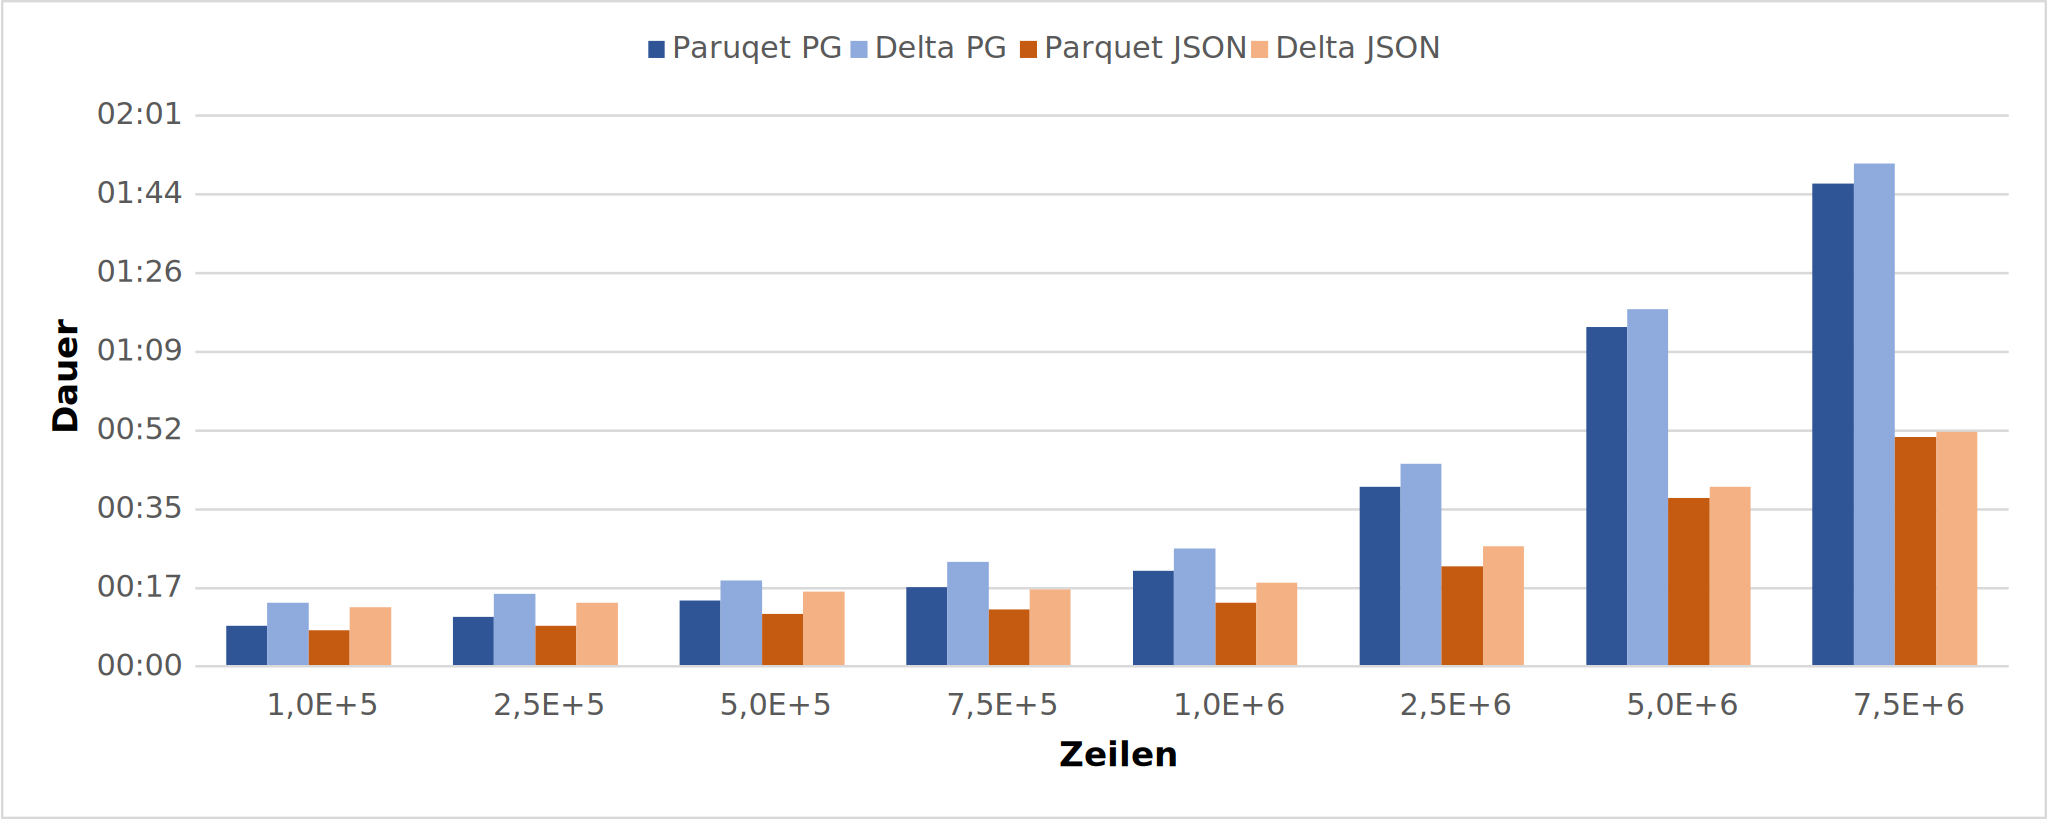
\includegraphics[width=\textwidth]{Grafiken/Evaluierung/Zeit-Initial}
    \label{fig:eval-time-i}
\end{figure}

\begin{figure}
    \centering
    \caption{Dauer Ingestion aus aktualisierten Daten}
    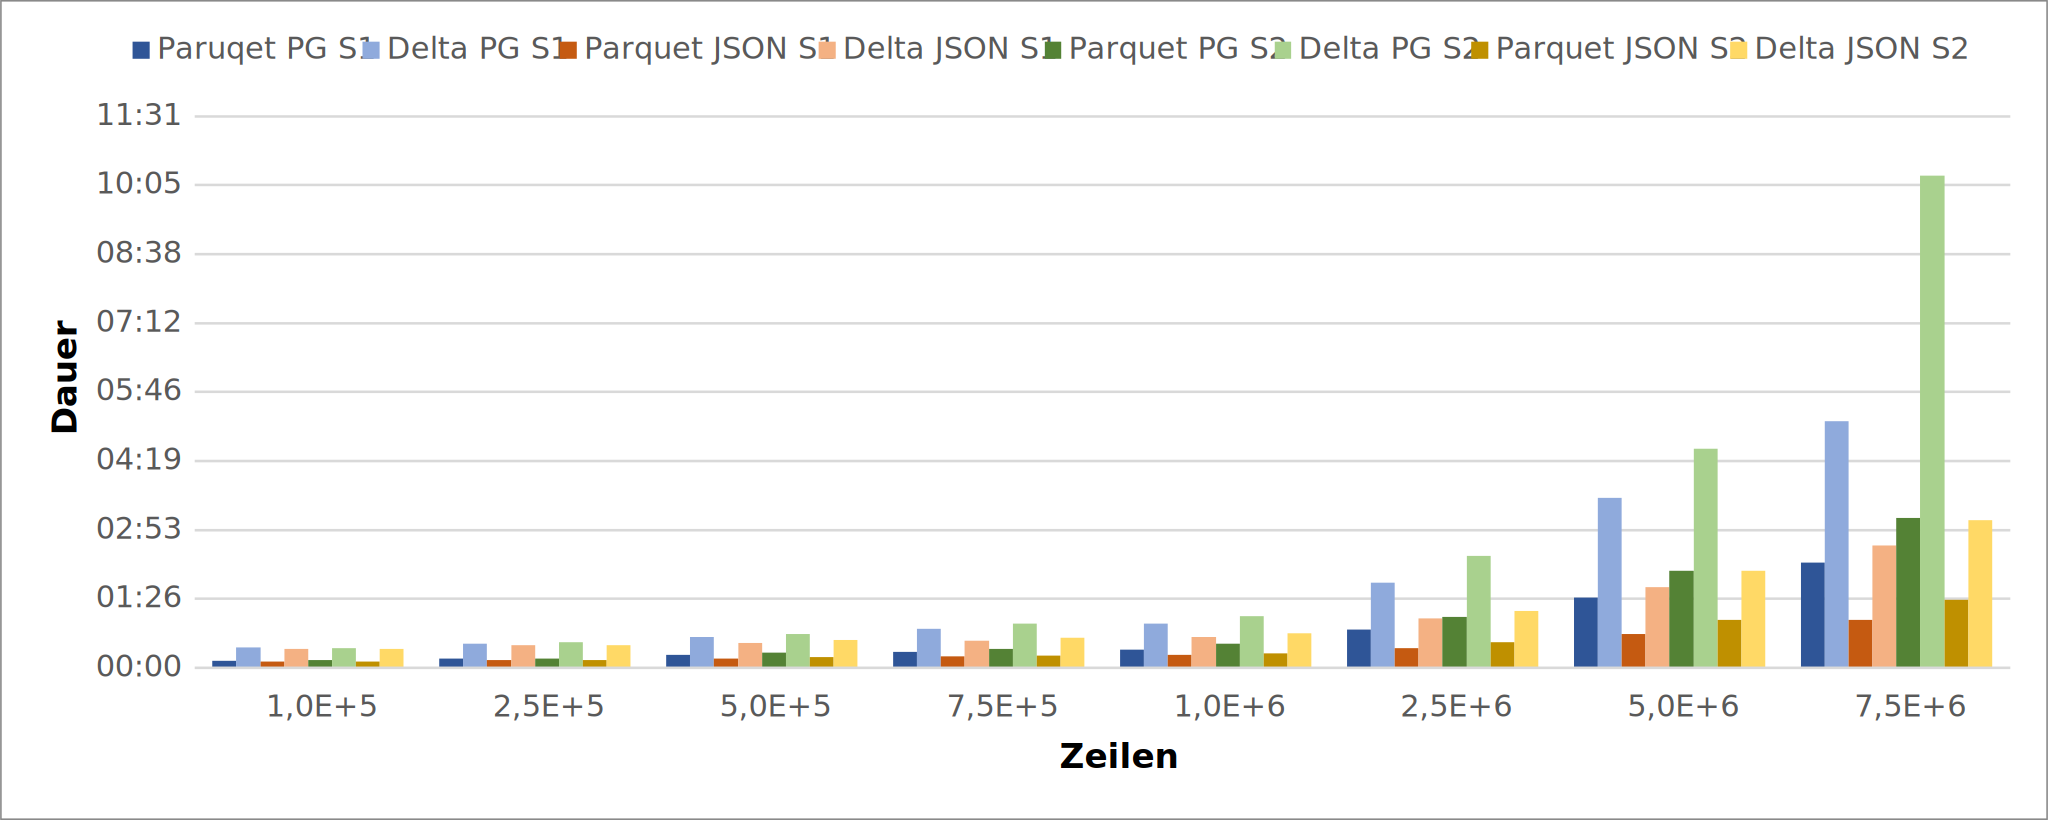
\includegraphics[width=\textwidth]{Grafiken/Evaluierung/Zeit-Update}
    \label{fig:eval-time-u}
\end{figure}

\begin{figure}
    \centering
    \caption{Dauer Ingestion aus Update-Quelle}
    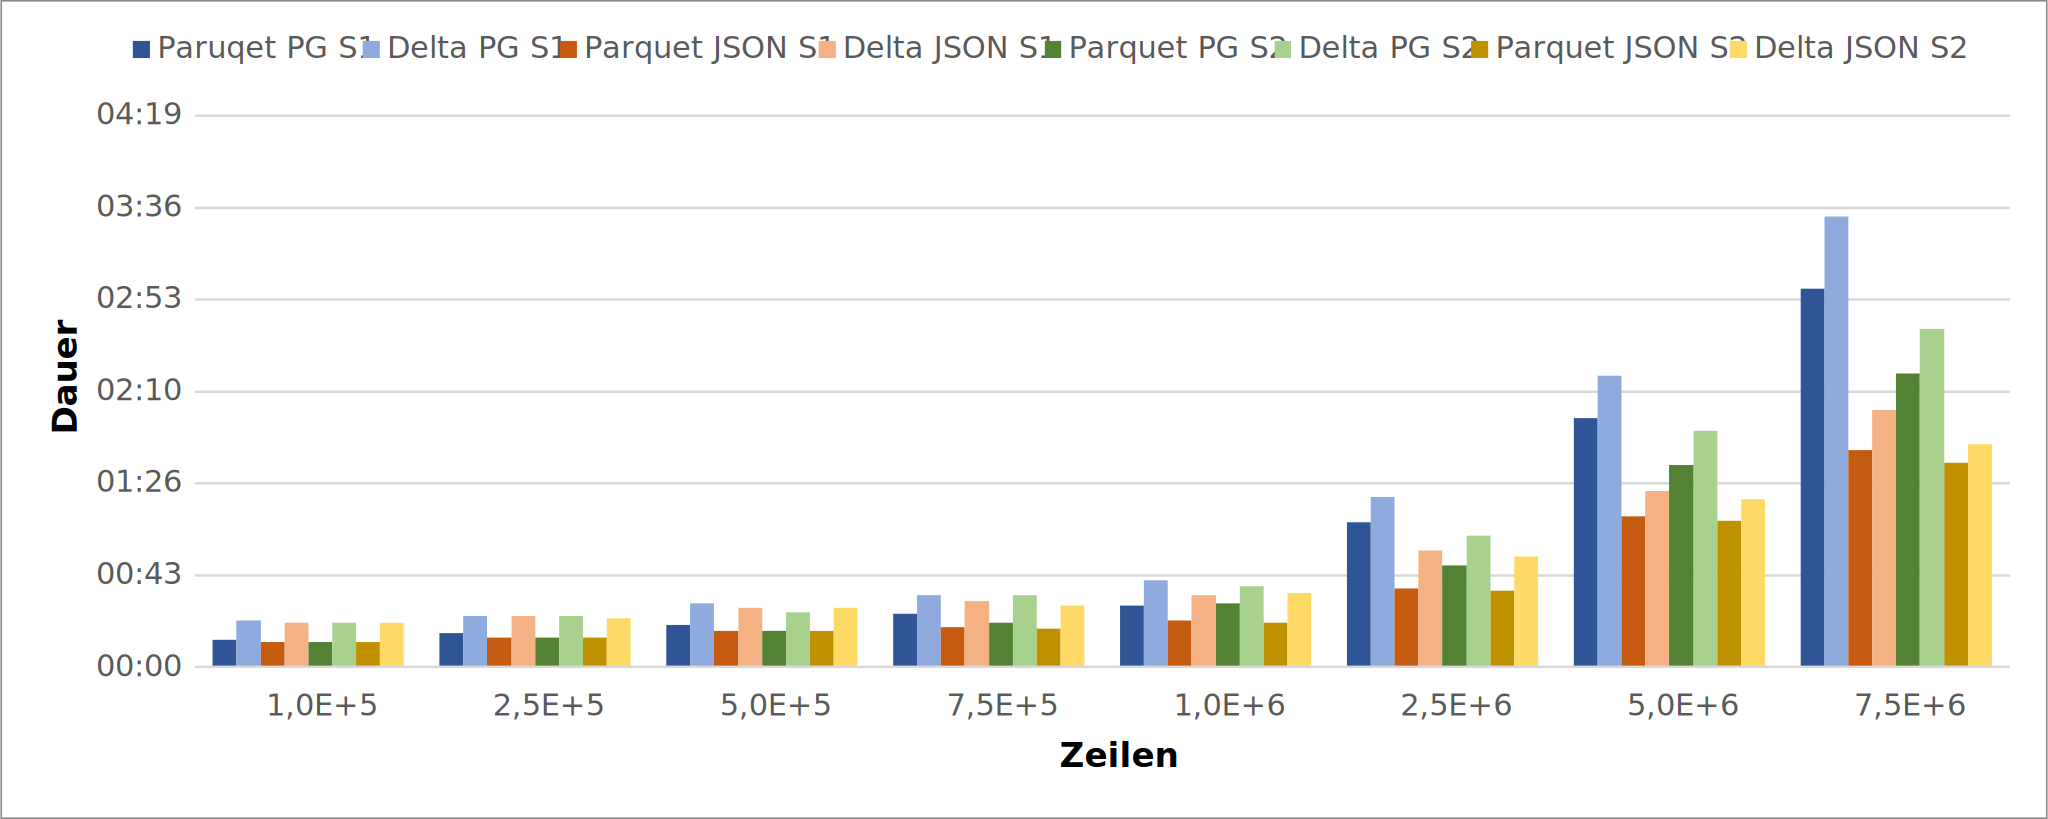
\includegraphics[width=\textwidth]{Grafiken/Evaluierung/Zeit-Cdc}
    \label{fig:eval-time-c}
\end{figure}

\subsubsection{Festplattenspeicherverbrauch}

Für die initiale Ingestion \cref{fig:eval-storage-i} ist kein Unterschied im Festplattenspeicherverbrauch zu erkennen.
Bei Betrachtung der genauen Werte ist zu sehen, dass die Delta-Tabellen einen leicht höheren Festplattenspeicherverbrauch haben.
Das liegt daran, dass Delta-Tabellen die Daten auch in Parquet speichern und nach der ersten Ingestion noch keine Versionierungsinformationen vorhanden sind.
Diese treten erst bei einer weiteren Ingestion auf.

Bei einer Ingestion von aktualisierten Daten (\cref{fig:eval-storage-u}) und aus einer Update-Quelle (\cref{fig:eval-storage-c}) ist der Festplattenspeicherverbrauch gleich.
Beide Quellen enthalten die gleichen Änderungen, weshalb auch das gespeicherte Ergebnis gleich sein muss.
Der Unterschied zwischen den Szenarien liegt darin, dass im zweiten Szenario mehr Daten eingefügt und weniger gelöscht werden, so dass am Ende mehr Daten im Datensatz enthalten sind.

Auch beim Festplattenspeicherverbrauch kommt die Eigenschaft der verschachtelten Daten in Spark zum Tragen.
Man sieht, dass weniger Spalteninformationen gespeichert werden müssen, was den Verbrauch niedriger hält.
Daraus lässt sich aber auch schließen, dass ohne weitere Verarbeitung weniger Informationen über Änderungen vorhanden sind.
Das heißt, dass bei Änderungen in einem verschachtelten Feld nur erkannt wird, dass sich das Feld auf der obersten Ebene darüber verändert hat.
Die genauen Änderungen müssen, durch zum Beispiel einen Vergleich der Versionen, nachträglich berechnet werden.


\begin{figure}
    \centering
    \caption{Festplattenspeicherverbrauch nach der ersten Ingestion}
    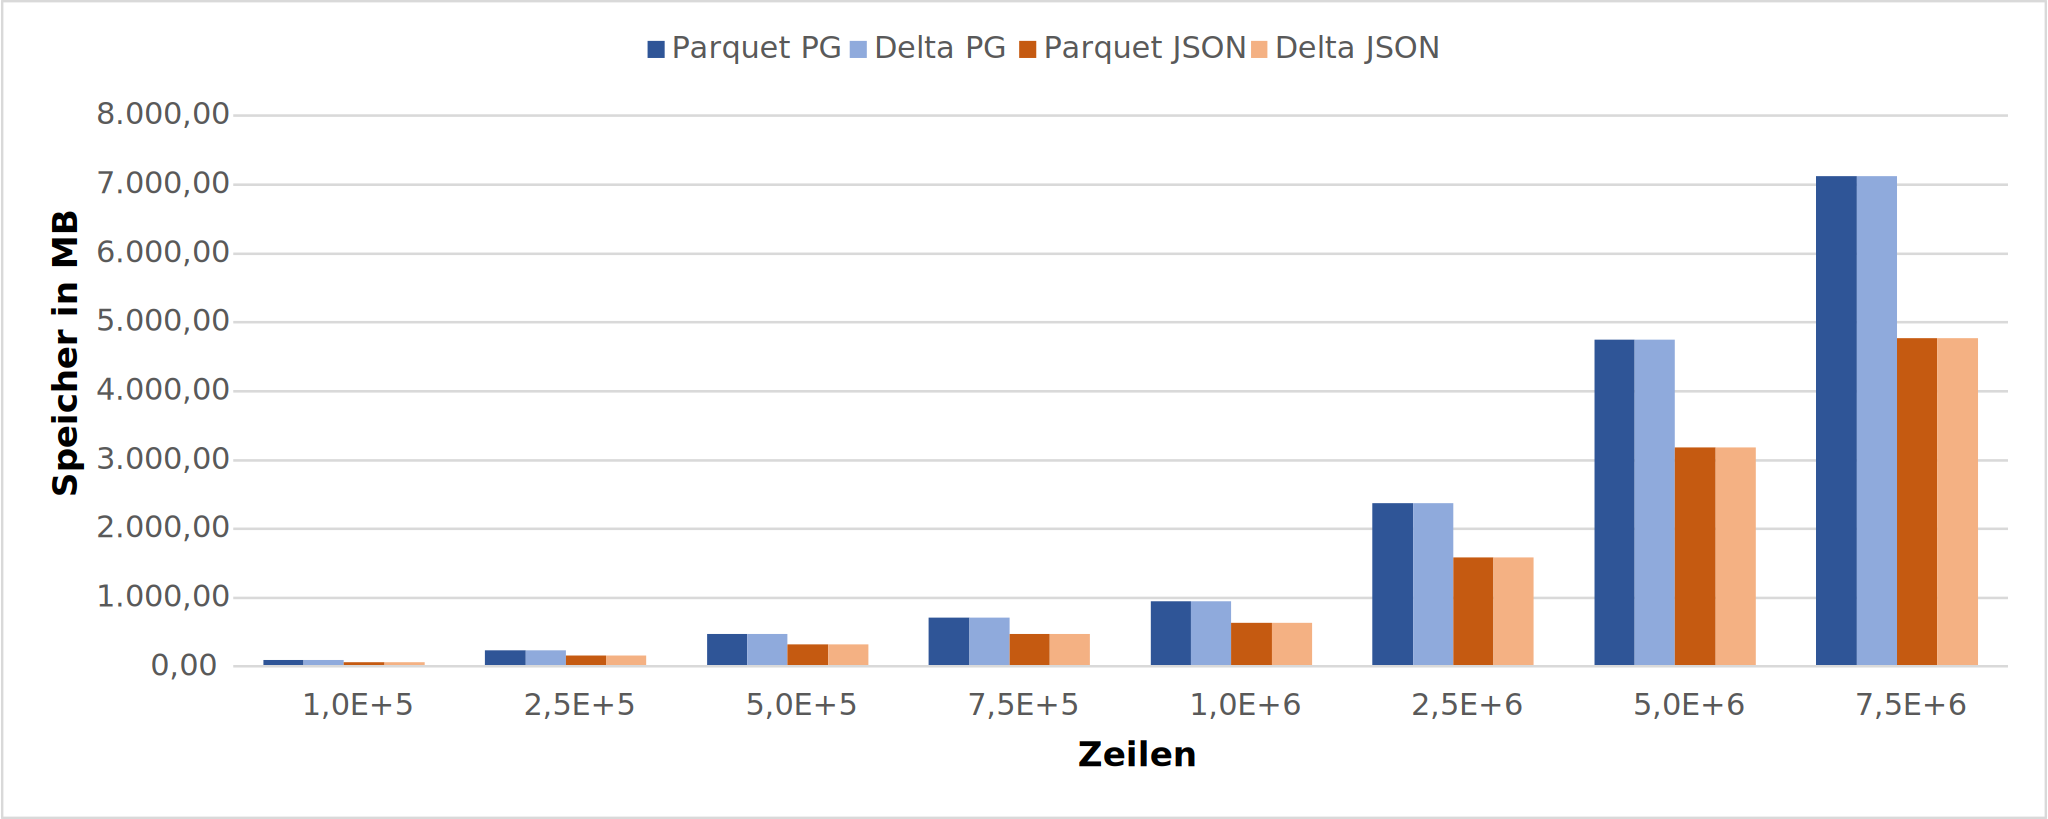
\includegraphics[width=\textwidth]{Grafiken/Evaluierung/Speicher-Initial}
    \label{fig:eval-storage-i}
\end{figure}

\begin{figure}
    \centering
    \caption{Festplattenspeicherverbrauch nach der Ingestion aus aktualisierten Daten}
    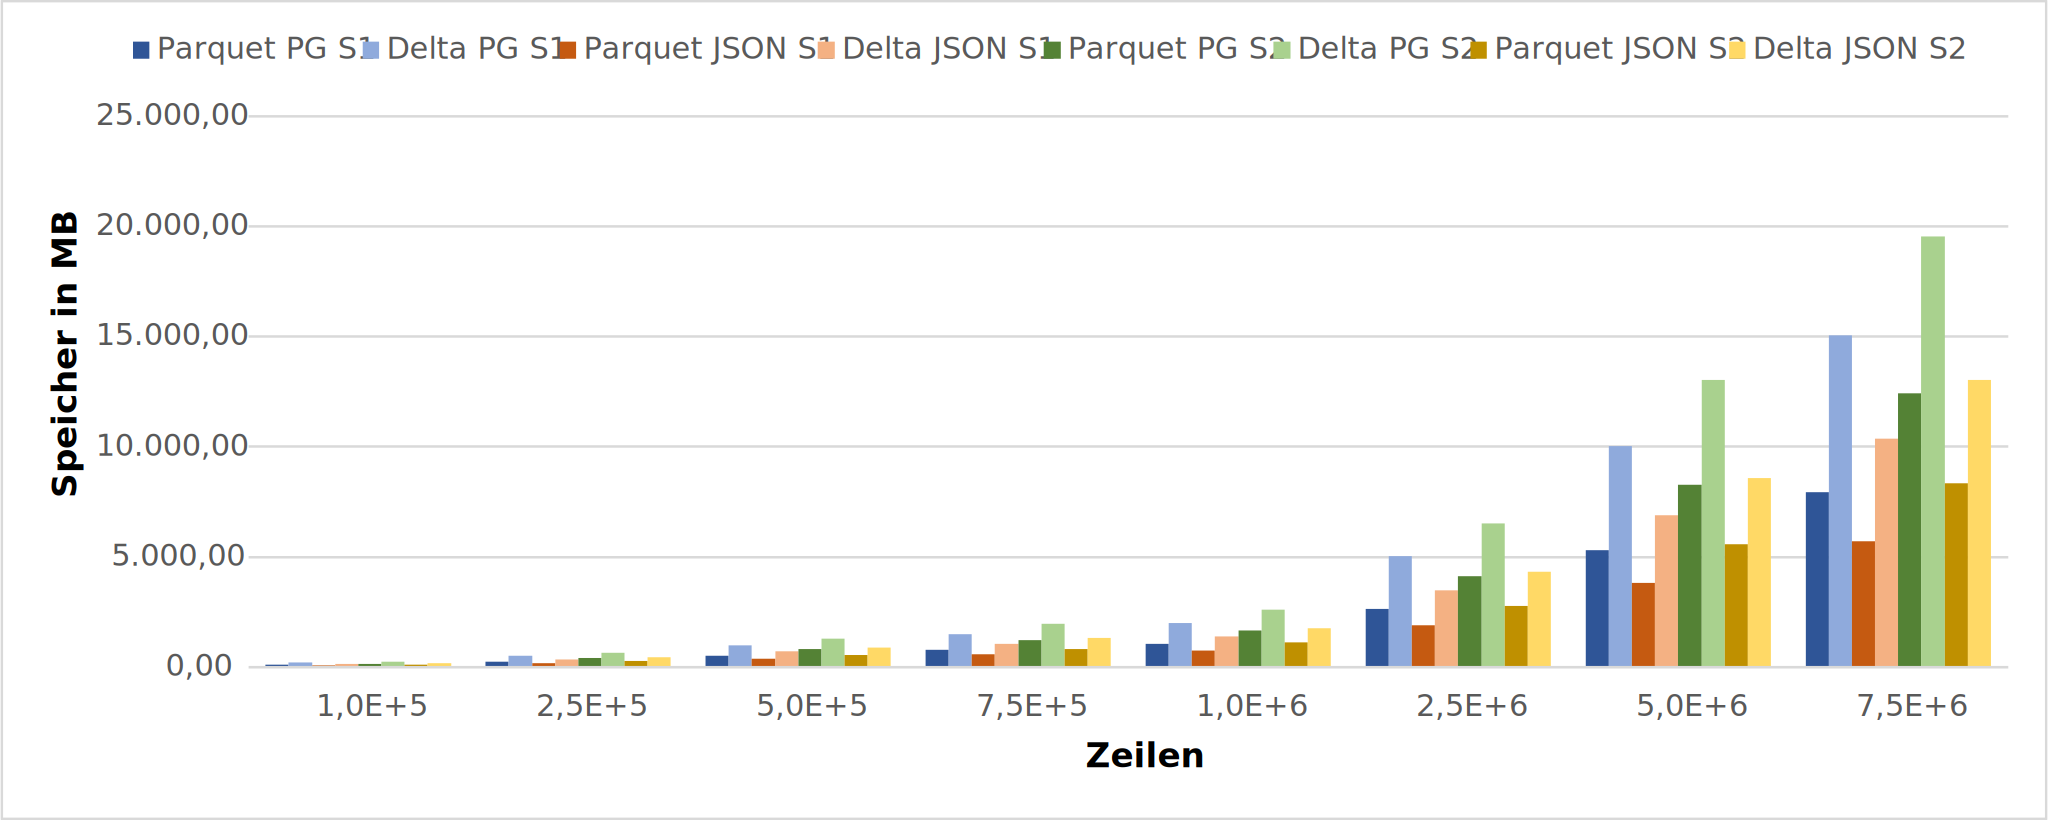
\includegraphics[width=\textwidth]{Grafiken/Evaluierung/Speicher-Update}
    \label{fig:eval-storage-u}
\end{figure}

\begin{figure}
    \centering
    \caption{Festplattenspeicherverbrauch nach der Ingestion aus Update-Quelle}
    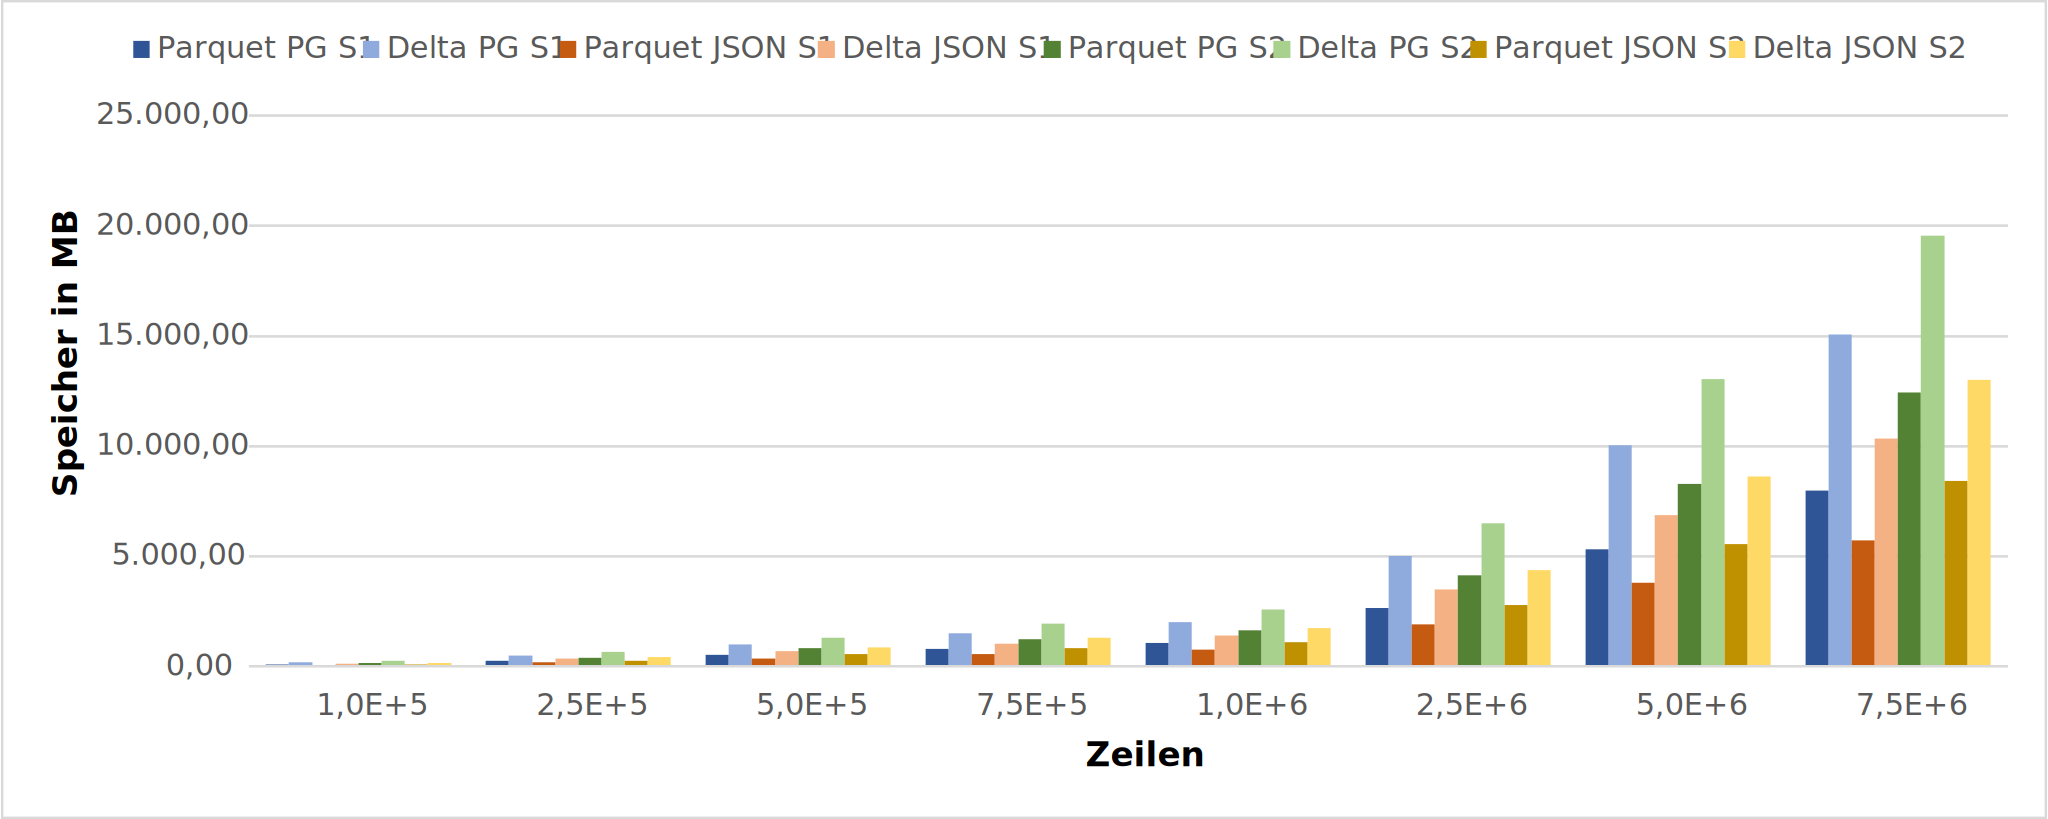
\includegraphics[width=\textwidth]{Grafiken/Evaluierung/Speicher-Cdc}
    \label{fig:eval-storage-c}
\end{figure}